
\chapter{Data Exploration}
\section{Introduction}
\paragraph{}
A good starting point for the analysis is to make some data exploration of the data set. The first thing to be done is statistical analysis such as counting the number of text per class or counting the number of words per sentence. The second step consit of doing Latent Dirichlet Allocation\cite{blei2003latent} in order to make unsupervised clustering of the text and see if there is some kind of correlation between the clusters to which a text belongs and its labels. 

\section{Dataset statistics}
\subsection{Fake News Corpus}
\paragraph{} Because \textbf{Fake News Corpus} is the main dataset, the data exploration will start with this dataset. And the first thing is to count the number of items per class. 

\paragraph{} Because the dataset have been cleaned, numbers provided by the dataset creators and number computed after cleaning will be provided. We found the values given at \textbf{Table \ref{tab:explo:count1}}. It shows that the number of fake news is smaller by a small factors with respect to the number of reliable news, but given the total number of items it should not cause any problems. But it will still be taken into account later on. 

\begin{table}[h]
\centering
	\begin{tabular}{l|r|r}
  Type & Provided & Computed\\
  \hline
  Fake News & $928,083$ & \\
  Satire & $146,080$ & \\
  Extreme Bias & $1,300,444$ & \\
  Conspiracy Theory & $905,981$ & \\
  Junk Science & $144,939$ & \\
  Hate News & $117,374$ & \\
  Clickbait & $292,201$ & \\
  Proceed With Caution & $319,830$ & \\
  Political & $2,435,471$ & \\
  Credible & $1,920,139$ & \\
  \hline
\end{tabular}
  \caption{Number of texts per categories}
  \label{tab:explo:count1}
\end{table}

\paragraph{} To have a better view of the distribution of categories, an histogram is provided at \textbf{Figure \ref{fig:chap1:hist1}}.

\begin{figure*}[h]
	\centering
	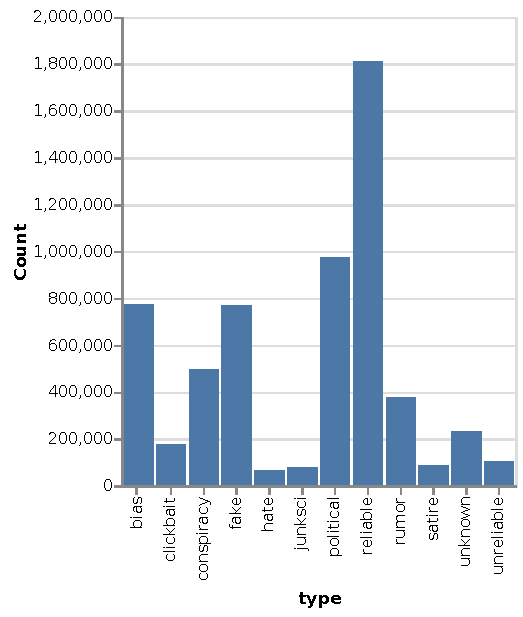
\includegraphics[width=0.5\textwidth]{chapter/images/data_exploration/plot1}
	\caption{Histogram of text distribution along their categories on the computed numbers. }
	\label{fig:chap1:hist1}
\end{figure*}
